\documentclass{article}
\usepackage[utf8]{inputenc}
\usepackage{enumitem}
\usepackage{nameref}

\usepackage{graphicx}
\usepackage{rotating}
\usepackage{epstopdf}


\usepackage{hyperref}
\hypersetup{
    colorlinks,
    citecolor=black,
    filecolor=black,
    linkcolor=black,
    urlcolor=black
}
\usepackage[dvipsnames]{xcolor}
\usepackage{listings}
\usepackage{alloy-style}

\begin{document}

\begin{figure}[t]
\centering
	
\includegraphics[height=6.25cm,keepaspectratio]{Figures/logo}
\end{figure}

\title{TrackMe \\ Software Engineering 2 Project\\ \textit{RASD Document} }
\author{Stefano Martina, Alessandro Nichelini, Francesco Peressini
		\\ \\ A.Y. 2018/2019}
		
\maketitle
\newpage

\tableofcontents
\newpage

\section{Introduction}

\subsection{Purpose} 

TrackMe is a company aiming to support interactions between users, 
who like keeping track of their health status and activities, and
third-parties, which can use data and enhance their value.


TrackMe app is composed of a core service: 
\begin{itemize}
\item Data4Help: which provides basic support for health and location data retrieving and sharing.
\end{itemize}

and two advanced services which relay on the first one.

\begin{itemize}

\item AutomatedSOS: add support for SOS services to elderly people;
\item Track4Run: add support for running events.
\end{itemize}

\begin{figure}[h!]
  \centering
  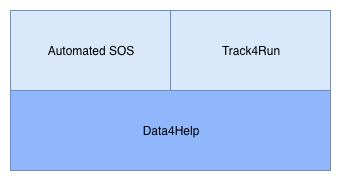
\includegraphics[height=4.5cm,keepaspectratio]{Figures/Services.png}
  \caption{Services abstract structure.}
\end{figure}

The project consists of a platform divided in a mobile application and a web-based interface to
serve third-parties.

The system allows individual users to add and handle data on the app
and to third-parties to request and have access to these data.

In particular, a user of the application is able to keep track of 
his/her position during the activities but also during the normal 
day-life. The users’ data are used to monitor the heartbeat and 
eventually to send an AutomatedSOS.
Furthermore, TrackMe, is able to track all the athletes (that are 
using the application), during a run previously organised. 
Indeed TrackMe’s app provides a section to setup a group run, 
specifying the path and other useful information.

\newpage
\subsection{Scope}
\subsubsection{Description of the problem}
Nowadays a lot of people track their activities with smartphone or
wearable devices. For this reason TrackMe provides a new complete user 
experience allowing all the users to read briefly the information
about all their activities history.
It also provides a service to organise a group run, during which
it’s possible to monitor all the athletes information.
Furthermore all the users are monitored and, in case of some trouble, 
an SOS will be launched .
\subsubsection{World Phenomena}
\begin{itemize}
	\item \textit{General user’s health condition}: the machine doesn’t know the information about possible user’s disease.
	\item \textit{First aid services status}: the machine doesn’t know the actual first aid services status.
	\item \textit{Overall third parties knowledge status}: the machine doesn’t know which informations third parties already have about users.
\end{itemize}

\subsubsection{Machine Phenomena}
\begin{itemize}
	\item \textit{Third-parties registration}
	\item \textit{User's registration}
	\item \textit{Data anonymisation}
\end{itemize}

\subsubsection{Shared Phenomena}
\begin{itemize}
	\item \textit{Vital parameters}: the machine can read vital parameters of the user such as BPM
	\item \textit{User's location}: the machine knows or can read actual and past user’s location
\end{itemize}

\subsubsection{Goals} \label{goals}
\begin{enumerate}[label={\textbf{[G\arabic*]}}]
\item Users can be recognised by their credentials. \label{g1}
\item Allow users to keep track of their health data.
\item Allow users to have access to an overview of their data, including health parameters and performed activities. \label{g3}
\item Allow users to manage their data access policy.
\item Allow users to monitor their performance during run workouts.
\item Each time vital signs go below a threshold value, first aid services have to be notified.
\item Allow users to organise running events.
		\begin{enumerate}[label={[G\arabic{enumi}.\arabic*]}]
    		\item Allow users to create running events.
    		\item Allow users to en-roll to events.
    		\item Allow spectators to follow participants’ live position during events.
  		\end{enumerate}
\item Allow third parties to access data:
		\begin{enumerate}[label={[G\arabic{enumi}.\arabic*]}]
    		\item Allow third parties to require access to specific user data.
    		\item Allow third parties to retrieve anonymised aggregated data.
    		\item Allow third parties to subscribe to data feed 
  		\end{enumerate}

\end{enumerate}

\newpage
\subsection{Definitions, Acronyms, Abbreviations}

\subsubsection{Definitions}
\begin{itemize}
	\item \textbf{Event:} An event organised by a user.
	\item \textbf{Notification:} A warning that advise the user of a request by third parties.
	\end{itemize}

\subsubsection{Acronyms}
\begin{itemize}
\item API: Application Programming Interface;
\item ASOS: AutomatedSOS;
\item BPM: Beats Per Minutes;
\item D4H: Data4Help;
\item T4R: Track4Run.
\end{itemize}

\subsubsection{Abbreviations}
\begin{itemize}
		\item \begin{math}[Gn]\end{math}: n-th goal
		\item \begin{math}[Dn]\end{math}: n-th domain assumption 
		\item \begin{math}[Rn]\end{math}: n-th functional requirement
\end{itemize}

\subsection{Revision history}
\begin{itemize}
	\item 1.0.0 Initial version (10/11/2018)
\end{itemize}
\subsection{Document Structure}
This document essentially follows the structure defined by IEEE for RASD document (\textit{ISO/IEC/IEEE 29148 dated Dec 2011}).

\newpage
\section{Overall description}

\subsection{Product perspective}
\subsubsection{Class Diagram}
The product perspective of TrackMe is now explained using the UML paradigms.
The main classes of the UML are:
\begin{itemize}
	\item \textbf{User} contains all the information about a user like username, password, fiscalCode, hometown, elderly, runners.
	\item \textbf{ThirdParties} contains all the information about the registered organisation.
	\item \textbf{Data} is an abstract class that has two concrete classes: 
		\textbf{Health data} and	 \textbf{Location data}
	\item \textbf{Running Event} 
	\item \textbf{Location} contains information like the start point and the end point of a running event.
\end{itemize}

A user creates an Event specifying the path ie the starting location, the ending location and some specific interesting point along the path.
After the creation some user can join in.
An organisation, as explained above, can subscribe to a feed of data or directly to a single user.


\begin{figure}[h!]
  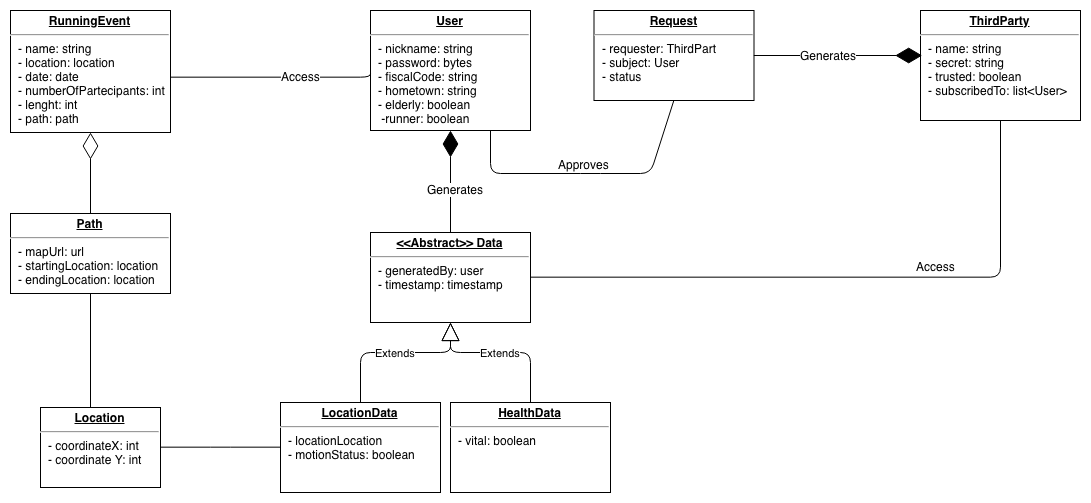
\includegraphics[width=\textwidth]{Figures/ClassDiagram.png}
  \caption{UML diagrams.}
\end{figure}
\newpage

\subsubsection{State Diagram}
The whole system can be also seen as a set of different services relying on the main module Data4Help.
Here we describe the main aspects of them with state diagrams.

\begin{figure}[h!]
  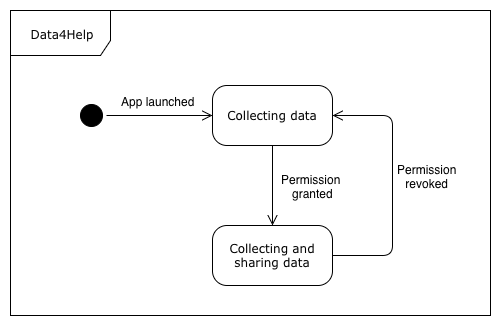
\includegraphics[width=\textwidth]{Figures/State1}
  \caption{Basic Data4Help service state diagram.}
  \label{fig:State1}
\end{figure}

\begin{figure}[h!]
	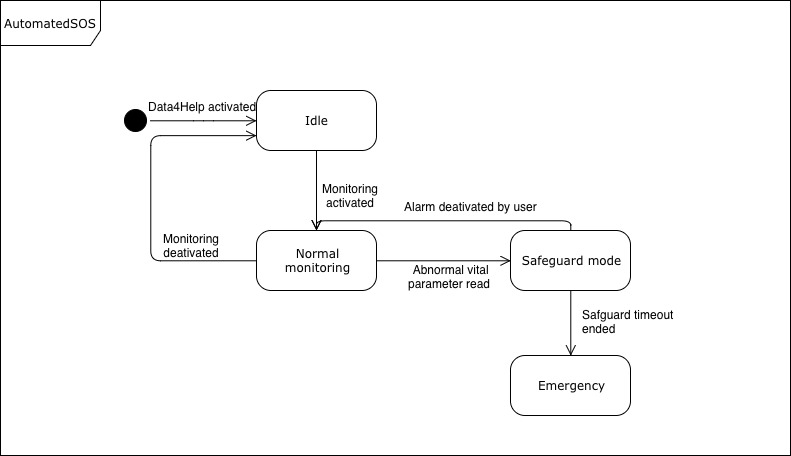
\includegraphics[width=\textwidth]{Figures/State2}
  \caption{Automated SOS state diagram.}
  \label{fig:State2}
\end{figure}

\newpage

\begin{figure}[h!]
  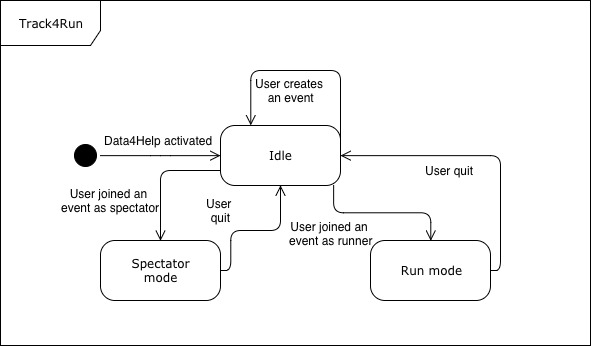
\includegraphics[width=\textwidth]{Figures/State3}
  \caption{Track4Run state diagram}
  \label{fig:State3.}
\end{figure}

\newpage

\subsection{Product functions}
The software developed by TrackMe include three different services:
Data4Help supports user's data acquisition through wearable devices, AutomatedSOS, a personalised and non-intrusive SOS 
service for elderly people and Track4Run, a service to track athletes 
participating to a run.
Data4Help is also a service available for third-parties: in fact, 
organisations can request data to TrackMe and collect them for 
pursuing their objectives.
Data acquisition can be performed in two different way: directly to a
single user or to a groups of individuals.
Concerning the single user case, companies, through a social security
code, ask permission to access the corresponding information. 
In the other case, organisations can request, directly to TrackMe,
data of group of individuals with particular properties (e.g. users 
between 20 and 30 years old or living in a certain district).
In the latter, TrackMe provides data only if it can anonymised them
correctly.
AutomatedSOS it’s great for those elderly people who want to monitor 
their health status and have the support of an ambulance in case their
vital parameters are under certain thresholds.
Track4Run it’s a service dedicated to the runners: it offers the 
possibility to organise a run between other runners, define the path 
and the duration, allowing the invited ones to en-roll. In addition, 
Track4Run users who do not partecipate to the run can see live time 
on a map the position of all the runners. 
Finally, Track4Run supports the synchronisation of data with 
Data4Help.

All the goals presented in section \ref{goals} are going to be 
implemented. Here we describe deeply the requirements needed to
implement application's functions.
	
\begin{enumerate}[label={[R\arabic*]}]
    	\item Users can create an account with credentials.
    	\item Credentials can be retrievable also if forgotten/lost.
    	\item Users can log manually or automatically their data.
    	\item Users have to be able to accept/deny access to single data access request.
    	\item Users have to be able to see current data policies and to change them.
    	\item The machine has to be able to read health and position data.
		\item The machine has to be able to recognise below threshold parameters.
		\item The machine has to be able to communicate with third parties.
		\item The machine has to be able to recognise data fragmentation level.
		\item The machine has to be able to store users’ data. 
\end{enumerate}
\newpage
\subsection{Users characteristics}
\textbf{Users}: any person that will use the service to keep track of health data, positioning or automated SOS during any kind of activities (walking or running during a lone run or an organised event).\\\
\textbf{Third-parties}: Organisation or other parties interested in the acquisition for their usage of the data provided by the user activities.

\subsection{Assumptions, dependencies and constraints}

\subsubsection{Domain assumptions}

\begin{enumerate}[label={[D\arabic*]}]
    	\item Data manually inserted by users are to be considered 
    	truthful   
    	\begin{enumerate}[label={[D\arabic{enumi}.\arabic*]}]
    			\item Data are up to date.
    			\item Data are correctly formatted.
  		\end{enumerate}

    	\item First aid services are ready to handle emergency notifications.  		
  		\item Running paths proposed by users are well formed (e.g: legit by law).
  		\item External services are reliable (map services).
  		\item Users can be localised trough GPS:
  		\begin{enumerate}[label={[D\arabic{enumi}.\arabic*]}]
    			\item GPS service is reliable.
    			\item GPS service is accurate enough to track runners during workouts.
  		\end{enumerate}
  		\item Users are not affected with diseases that can influence heartbeat ratio.
  		
\end{enumerate}

\newpage
\section{Specific Requirements}

\subsection{External Interface Requirements}

	\subsubsection{User Interfaces} 	
	
	\begin{figure}[!h]
	 	\centering
		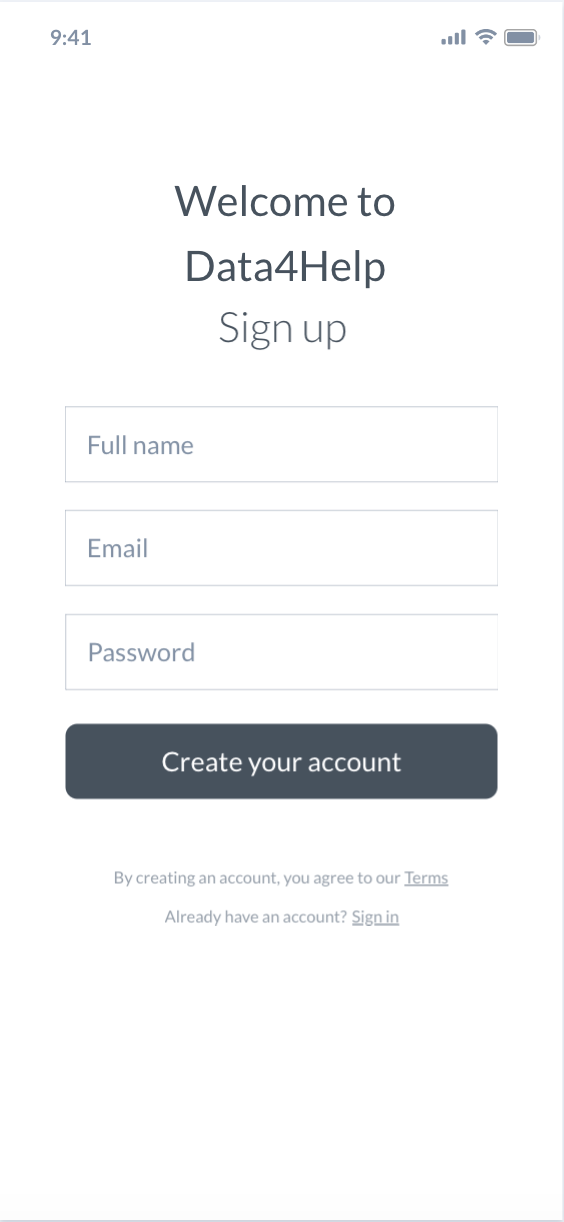
\includegraphics[height=15cm,keepaspectratio]{Figures/1SignUp}
		\caption{Sign Up}
	\end{figure}\newpage
	
	\begin{figure}[!h]
	 	\centering
		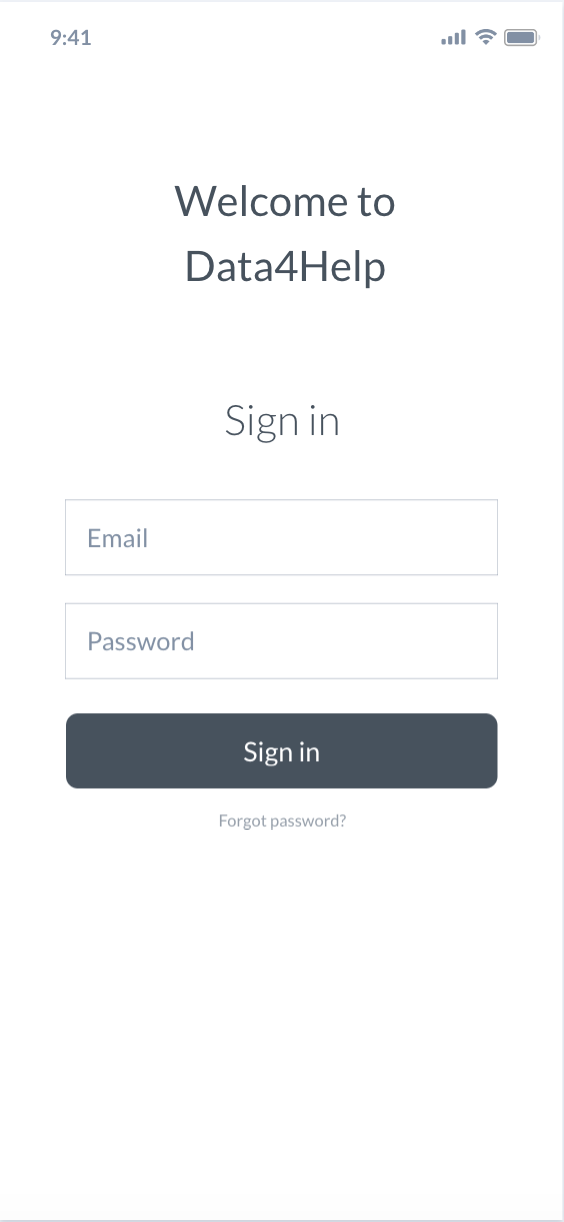
\includegraphics[height=15cm,keepaspectratio]{Figures/2SignIn}
		\caption{Sign In}
	\end{figure}\newpage
	
	\begin{figure}[!h]
	 	\centering
		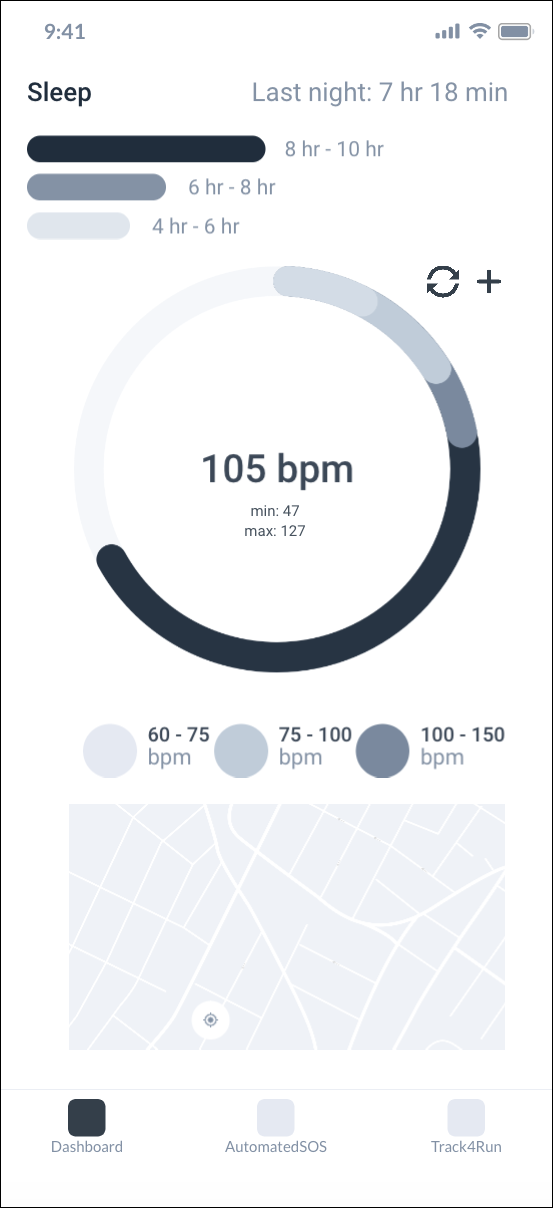
\includegraphics[height=15cm,keepaspectratio]{Figures/3Dashboard}
		\caption{Data4Help dashboard}
	\end{figure}\newpage
	
	\begin{figure}[!h]
	 	\centering
		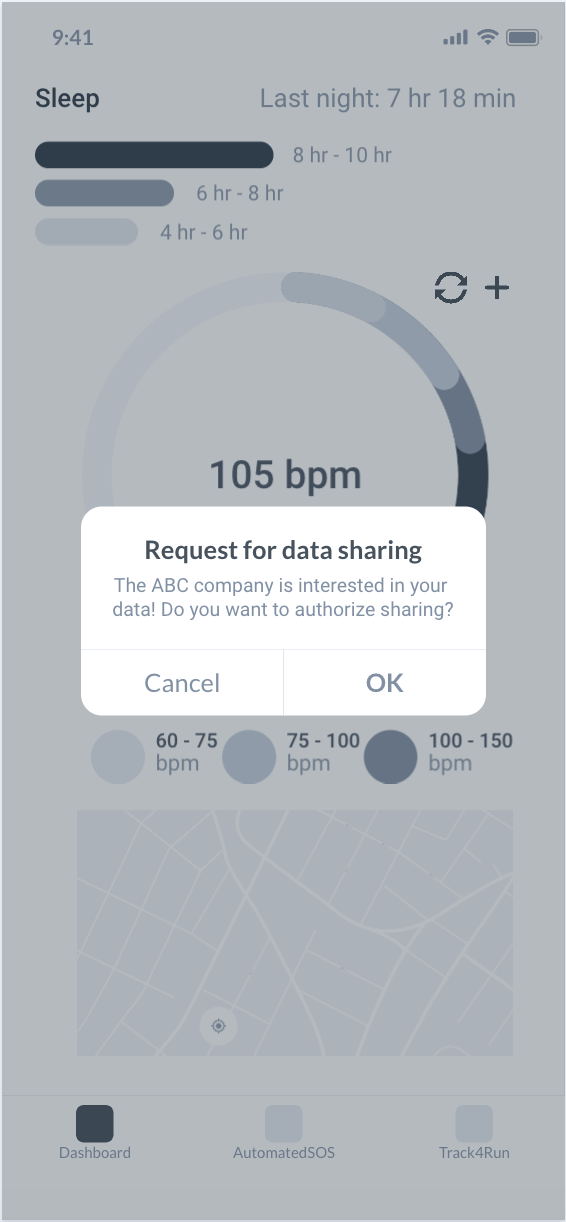
\includegraphics[height=15cm,keepaspectratio]{Figures/4DataSharing}
		\caption{Request for data sharing}
	\end{figure}\newpage
	
	\begin{figure}[!h]
	 	\centering
		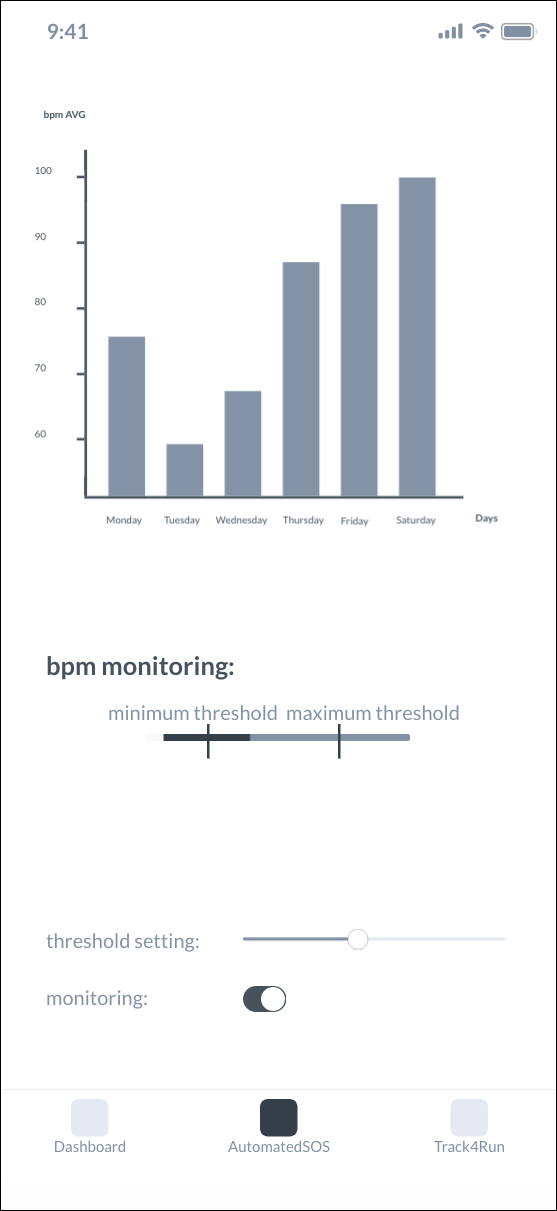
\includegraphics[height=15cm,keepaspectratio]{Figures/5AutomatedSOS}
		\caption{AutomatedSOS dashboard}
	\end{figure}\newpage
	
	\begin{figure}[!h]
	 	\centering
		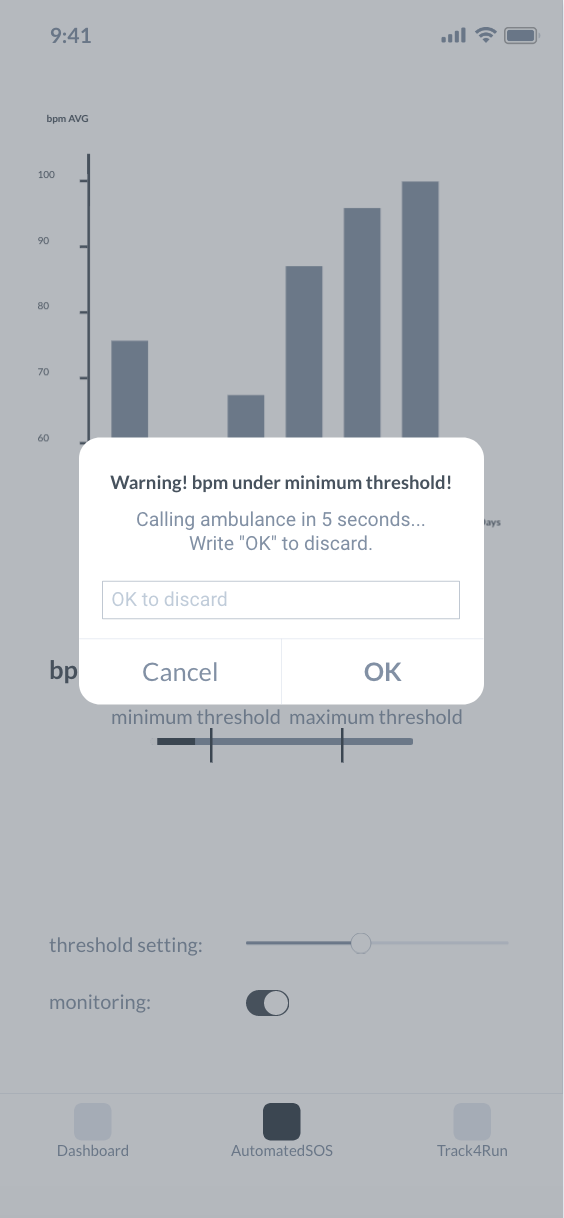
\includegraphics[height=15cm,keepaspectratio]{Figures/6Low}
		\caption{Emergency case}
	\end{figure}\newpage	
	
	\begin{figure}[!h]
	 	\centering
		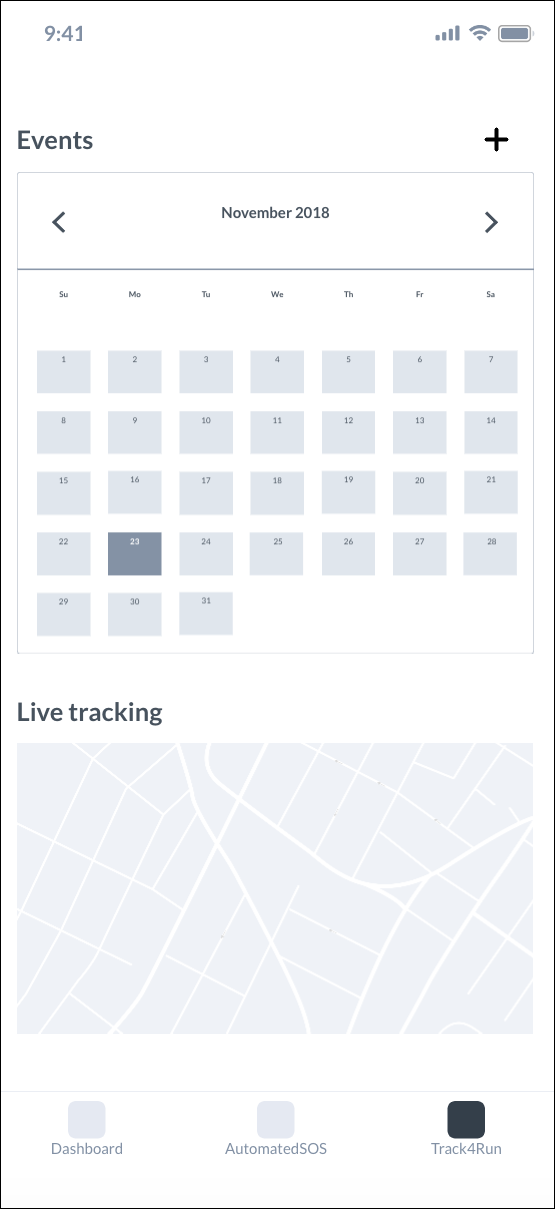
\includegraphics[height=15cm,keepaspectratio]{Figures/7Track4Run}
		\caption{Track4Run dashboard}
	\end{figure}\newpage	
	
	\begin{figure}[!h]
	 	\centering
		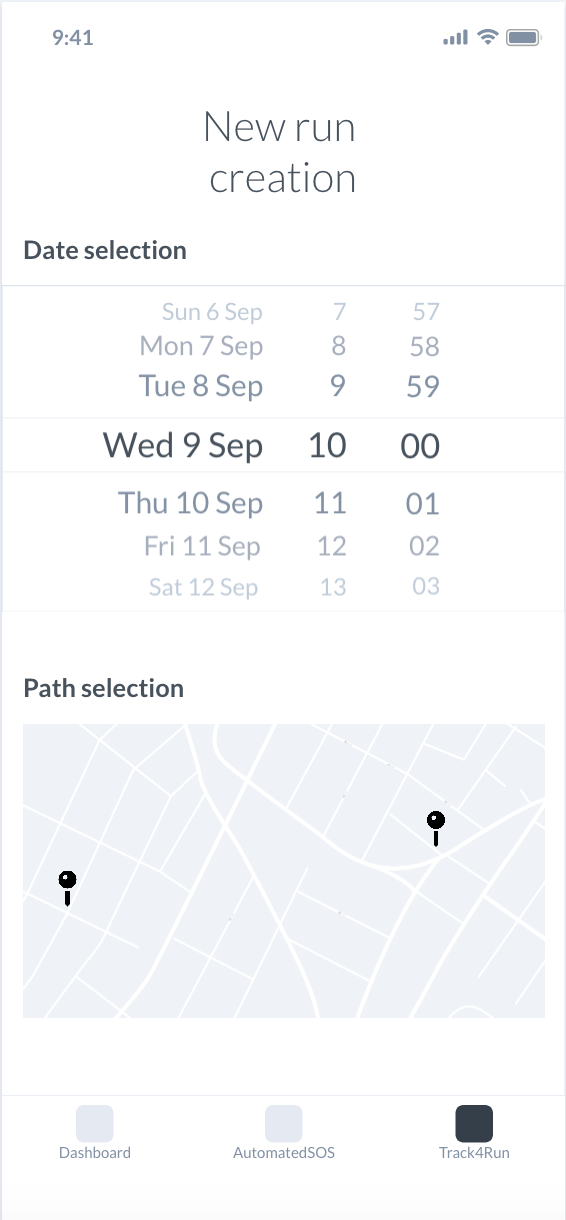
\includegraphics[height=15cm,keepaspectratio]{Figures/8Path}
		\caption{New run creation}
	\end{figure}\newpage	
	
	\newpage
	\subsubsection{Hardware Interfaces}
	TrackMe is a software application that does not export any 
	hardware interface; instead, at the final user is required a 
	smartphone and at the third-party is required a web browser. 
			
	\subsubsection{Software Interfaces}
	\begin{itemize}
		\item \textbf{Data4Help} \newline 
		User's health data can be inserted in Data4Help section of the
		application manually or automatically synchronised with data
		acquired by individual's wearable device. \newline
		Third-parties can access to the different data through a 
		web-based interface in which, in case the organisation is 
		interested in the information of some specific individual, 
		can select the single user by his/her fiscal code and send to
		him/her the request of data's visualisation; instead, in 
		case of interest in accessing data of groups of individuals, 
		companies can select the parameters of interest and send to 
		TrackMe the request on hold for a positive response.
		\item \textbf{AutomatedSOS} \newline
		Similarly as Data4Help, AutomatedSOS automatically 
		synchronises data acquired from user's wearable device and 
		monitors them to guarantee the safety of elderly people. 
		\newline
		In case of emergency, an ambulance will reach the location
		of the customer; moreover, AutomatedSOS allows to follow 
		live-time the position of the coming ambulance. 
		\item \textbf{Track4Run} \newline
		Since Track4Run aims to schedule and organise runs for the 
		users of the service, it makes use of an external calendar
		service to allow individuals to create and en-roll races. 
		\newline
		For those who do not participate to the runs, Track4Run 
		features the possibility to see live-time the position of
		the runners.
	\end{itemize} 
	
	\subsubsection{Communication Interfaces}
	The system is going to use an API based communication system to 
	serve both the mobile application and the third-parties. \newline
	Data will be exchanged in multi-platform data formats such as 
	JSON or XML.
		
\newpage
\subsection{Functional Requirements}	

Here we map each goal to the corresponding machine requirement(s) and 
world domain assumption(s) that have to be made in order to reach it.

\begin{itemize}	

	\item [G1] Users can be recognised by their credentials.
	\begin{itemize}
		\item [R1] Users can create an account with credentials.
		\item [R2] Credentials can be retrievable also if 
		forgotten/lost.
	\end{itemize} 

	\item [G2] Allow users to keep track of their health data.	
	\begin{itemize}
		\item [R3] Users can log manually or automatically their data.
		\item [R6] The machine has to be able to read health and 
		position data.
	\end{itemize}
	
	\item [G3] Allow users to have access to an overview of their 
	data, including health parameters and performed activities.
	\begin{itemize}
		\item [R10] The machine has to be able to store users’ data.
	\end{itemize}
	
	\item [G4] Allow users to manage their data access policy.
	\begin{itemize}
		\item [R4] Users have to be able to accept/deny access to 
		single data access request.
		\item [R5] Users have to be able to see current data policies
		and to change them.
	\end{itemize}
	
	\item [G5] Allow users to monitor their performances during 
	workouts.	
	\begin{itemize}
		\item [D5] External services are reliable (map services).
		\item [D6] Users can be localised trough GPS.
	\end{itemize}	
	
	\item [G6] Each time vital signs go below a threshold value, first 
	aid services have to be notified.
	\begin{itemize}
		\item [R6] The machine has to be able to read health and 
		position data. 
		\item [R7] The machine has to be able to recognise below 
		threshold parameters.
		\item [D1] Data manually logged by users well describe 
		reality.
		\item [D3] First aid services are ready to handle emergency
		notifications.
		\item [D7]Users are not affected with diseases that can 
		influence heartbeat ratio.
	\end{itemize}
		
	\item [G7] Allow users to organise running events.
	\begin{itemize}
		\item [D4] Running paths proposed by users are well formed 
		(e.g: legit by law). 
	\end{itemize}
	
	\item [G8] Allow third parties to access data.
	\begin{itemize}
		\item [R8] The machine has to be able to communicate with 
		third parties. 
		\item [R9] The machine has to be able to recognise data 
		fragmentation level.
		\item [R10] The machine has to be able to store users’ data.
	\end{itemize}
	
\end{itemize}

\newpage
\subsubsection{Definitions of use cases}

\begin{table}[h!]
	\begin{tabular}{ | p{3cm} | p{12,5cm} | }
	\hline
	Name & Sign up \\ \hline
	Actor & User \\ \hline
	Entry conditions & The application has been correctly installed on user's device  \\ \hline
	Events flow & \begin{tabular}[c]{@{}l@{}}1. Select the "Sign up" option~\\2. Fill in all the fields necessary for registering to the services~\\3. Tap on the sign up button to confirm the inputted data\end{tabular} \\ \hline
	Exit conditions & \begin{tabular}[c]{@{}l@{}}Data has been successfully saved and the customer can now use ~~\\ all the services offered by the application~\end{tabular} \\ \hline
	Exceptions & \begin{tabular}[c]{@{}l@{}}1. User is already registered~\\2. User inputted email is already registered~\\3. User has chosen a username already taken\\4. Not all fields were correctly filled~\\5. User has to recompile the sign up module correcting the ~~\\ ~~~~invalid fields~\end{tabular}  \\ \hline
	\end{tabular}
	\caption{Sign up case}
\end{table}

\begin{table}[h!]
	\begin{tabular}{ | p{3cm} | p{12,5cm} | }
\hline
Name             & Log in                                                                                                                                                                                                                         \\ 
\hline
Actor            & User                                                                                                                                                                                                                           \\ 
\hline
Entry conditions & \begin{tabular}[c]{@{}l@{}}The installed application and the registration to the platform are ~~\\ mandatory to correctly log in~\end{tabular}                                                                                    \\ 
\hline
Events flow      & \begin{tabular}[c]{@{}l@{}}1. Select the "Log in" option~\\2. Fill in the "Username" and "Password" fields~\\3. Tap on the log in button to confirm the credentials~\end{tabular}                                              \\ 
\hline
Exit conditions  & \begin{tabular}[c]{@{}l@{}}User has been correctly identified by the system and redirected ~~\\ to the main page of the application~\end{tabular}                                                                                 \\ 
\hline
Exceptions       & \begin{tabular}[c]{@{}l@{}}1. User inputted an invalid username~\\2. User inputted an invalid password~\\3. User is not register to the platform~\\4. User has to correct the invalid fields of the log in page~\end{tabular}  \\
\hline
\end{tabular}
\caption{Log in use case}
\end{table}
\newpage

\begin{table}[h!]
\begin{tabular}{ | p{3cm} | p{12,5cm} | }
\hline
Name             & Manual data acquisition~                                                                                                                                                                                                                                                                                          \\ 
\hline
Actor            & User                                                                                                                                                                                                                                                                                                              \\ 
\hline
Entry conditions & \begin{tabular}[c]{@{}l@{}}The application has to be correctly installed and~\\the user has to be logged in~\end{tabular}                                                                                                                                                                        \\ 
\hline
Events flow      & \begin{tabular}[c]{@{}l@{}}1. Open the application and select the Data4Help section\\2. Tap the "Insert" button to manually insert data into the ~\\ ~~~~application~\\3. Confirm the inserted data by tapping the "Confirm" button\\4. Wait until the data inserted are correctly processed by the ~\\  ~~~~server~\end{tabular}  \\ 
\hline
Exit conditions  & Data are correctly updated and visible inside the application~                                                                                                                                                                                                                                                    \\ 
\hline
Exceptions       & \begin{tabular}[c]{@{}l@{}}1. Network error during the insertion phase~\\2. Inserted data are out-of-date\\3. User is invited to update the inserted information or to try ~\\ ~~~~again later~\end{tabular}                                                                                                        \\
\hline
\end{tabular}
\caption{Manual data acquisition}
\end{table}

\begin{table}[h!]
\begin{tabular}{ | p{3cm} | p{12,5cm} | }
\hline
Name             & Automatic data acquisition~                                                                                                                                                                                                                                                                                                                 \\ 
\hline
Actor            & User                                                                                                                                                                                                                                                                                                                                        \\ 
\hline
Entry conditions & \begin{tabular}[c]{@{}l@{}}The application has to be correctly installed and the user has to ~\\ be logged in~\end{tabular}                                                                                                                                                                                                  \\ 
\hline
Events flow      & \begin{tabular}[c]{@{}l@{}}1. Open the application and select the Data4Help section\\2. If not already updated, tap on the "synchronise" button\\3. Wait until the synchronisation between the smartphone and ~\\ ~~~~the wearable device is completed \\4. Wait until the data inserted are correctly processed by the ~\\ ~~~~server~\end{tabular}  \\ 
\hline
Exit conditions  & Data are correctly updated and visible inside the application~                                                                                                                                                                                                                                                                              \\ 
\hline
Exceptions       & \begin{tabular}[c]{@{}l@{}}1. Network error during the insertion phase~\\2. Synchronisation problem between the smartphone and the ~\\ ~~~~wearable device~\\3. User is invited to check the connection between devices or ~\\ ~~~~to try again later~\end{tabular}                                                                             \\
\hline
\end{tabular}
\caption{Automatic data acquisition}
\end{table}
\newpage

\begin{table}[h!]
\begin{tabular}{ | p{3cm} | p{12,5cm} | }
\hline
Name             & Specific-individual data request~                                                                                                                                                                                    \\ 
\hline
Actor            & Third-party~                                                                                                                                                                                                         \\ 
\hline
Entry conditions & The third-party has to be logged in on the TrackMe's web service page~                                                                                                                                               \\ 
\hline
Events flow      & \begin{tabular}[c]{@{}l@{}}1. Select from the web page the interested individual by his/her fiscal code\\2. Send a request for data sharing to the individual~\\3. Wait for the individual's response~\end{tabular}  \\ 
\hline
Exit conditions  & \begin{tabular}[c]{@{}l@{}}Customer has accepted the third-party request and the latter is now in possession~\\of the individual's information~\end{tabular}                                                         \\ 
\hline
Exceptions       & \begin{tabular}[c]{@{}l@{}}1. Network error during the request phase\\2. Negative response by the customer~\\3. The third-party is invited to try with another individual or to try again later\end{tabular}         \\
\hline
\end{tabular}
\caption{Specific-individual data request}
\end{table}

\begin{table}[h!]
\begin{tabular}{ | p{3cm} | p{12,5cm} | }
\hline
Name             & Groups-of-individuals data request~                                                                                                                                                                                                                         \\ 
\hline
Actor            & Third-party~                                                                                                                                                                                                                                                \\ 
\hline
Entry conditions & The third-party has to be logged in on the TrackMe's web service page~                                                                                                                                                                                      \\ 
\hline
Events flow      & \begin{tabular}[c]{@{}l@{}}1. Select from the web page the interested ~parameters for which the third-party\\~ ~ wants~to receive the data\\2. Wait for the~data-anonymisation control by TrackMe for the ~\\ ~~~~requested parameters~\end{tabular}                \\ 
\hline
Exit conditions  & \begin{tabular}[c]{@{}l@{}}TrackMe has ensured the anonymisation of the data and has accepted the \\third-party request; the latter is now in possession~of the individual's information~\end{tabular}                                                      \\ 
\hline
Exceptions       & \begin{tabular}[c]{@{}l@{}}1. Network error during the request phase\\2. Negative response by TrackMe (data-anonymisation control failed)~\\3. The third-party is invited to try with less restrictive parameters or to try again \\~ ~ later\end{tabular}  \\
\hline
\end{tabular}
\caption{Groups-of-individuals data request}
\end{table}
\newpage

\begin{table}[h!]
\begin{tabular}{ | p{3 cm} | p{12,5 cm} | }
\hline
Name             & Emergency situation~                                                                                                                                                                                                                                                                                                                                                          \\ 
\hline
Actor            & AutomatedSOS~                                                                                                                                                                                                                                                                                                                                                                 \\ 
\hline
Entry conditions & \begin{tabular}[c]{@{}l@{}}The application has to be correctly installed and\\the user has to be logged in~\end{tabular}                                                                                                                                                                                                                                     \\ 
\hline
Events flow      & \begin{tabular}[c]{@{}l@{}}1. The service automatically notice that one or more vital parameters are\\~ ~ under the safe threshold~\\2. The service asks to the customer if there are any problems with a pop-up\\~ ~ on-screen\\3. If the service doesn't receive a response within 5 seconds, an ambulance~\\~ ~ is alerted to reach the customer's location~\end{tabular}  \\ 
\hline
Exit conditions  & The ambulance reach the customer's location to take of him/her                                                                                                                                                                                                                                                                                                                \\ 
\hline
Exceptions       & \begin{tabular}[c]{@{}l@{}}1. Network error while contacting the ambulance service~\\2. The system keeps trying to reach the ambulance service until it succeeds or\\~ ~ the customer stops the process~\end{tabular}                                                                                                                                                         \\
\hline
\end{tabular}
\caption{Emergency situation}
\end{table}

\begin{table}[h!]
\begin{tabular}{ | p{3cm} | p{12,5cm} | }
\hline
Name             & Definition of a path~                                                                                                                                                                                                                                                                                                                                              \\ 
\hline
Actor            & User                                                                                                                                                                                                                                                                                                                                                               \\ 
\hline
Entry conditions & \begin{tabular}[c]{@{}l@{}}The application has to be correctly installed and\\the user has to be logged in~\end{tabular}                                                                                                                                                                                                                          \\ 
\hline
Events flow      & \begin{tabular}[c]{@{}l@{}}1. Open the application and select the Track4Run section~\\2. Tap on the "Create new run" button~\\3. Select the starting and ending points on the map\\4. Select the main spots of the path in order to define a complete route \\~ ~ on the map\\5. Wait until the data inserted are correctly processed by the server~\end{tabular}  \\ 
\hline
Exit conditions  & \begin{tabular}[c]{@{}l@{}}The path has been correctly defined by the customer and the run can be shared\\with the other users~\end{tabular}                                                                                                                                                                                                                       \\ 
\hline
Exceptions       & \begin{tabular}[c]{@{}l@{}}1. Network error during the definition of the path\\2. The starting/ending point or the main spots are not selectable~\\3. The path defined is not safe for the runners~\\4. The user is invited to redefine the path or to try again later\end{tabular}                                                                                \\
\hline
\end{tabular}
\caption{Definition of a path}
\end{table}
\newpage

\begin{table}[h!]
\begin{tabular}{ | p{3cm} | p{12,5cm} | }
\hline
Name             & Enrolment to a run~                                                                                                                                                                                                                         \\ 
\hline
Actor            & User                                                                                                                                                                                                                                         \\ 
\hline
Entry conditions & \begin{tabular}[c]{@{}l@{}}The application has to be correctly installed and\\the user has to be logged in~\end{tabular}                                                                                                    \\ 
\hline
Events flow      & \begin{tabular}[c]{@{}l@{}}1. Open the application and select the Track4Run section~\\2. Tap on the "Available runs" button to show all the forthcoming runs\\3. Select a run from those available and confirm the enrolment~\end{tabular}  \\ 
\hline
Exit conditions  & The user has correctly en-roll to the run                                                                                                                                                                                                    \\ 
\hline
Exceptions       & \begin{tabular}[c]{@{}l@{}}1. Network error during the enrolment~\\2. The run selected is no longer available/sold out\\3. The user is invited to choose another available run or to try again\\~ ~ later~\end{tabular}                     \\
\hline
\end{tabular}
\caption{Enrolment to a run}
\end{table}
\newpage

\subsubsection{Use case diagram}
\begin{figure}[h!]
  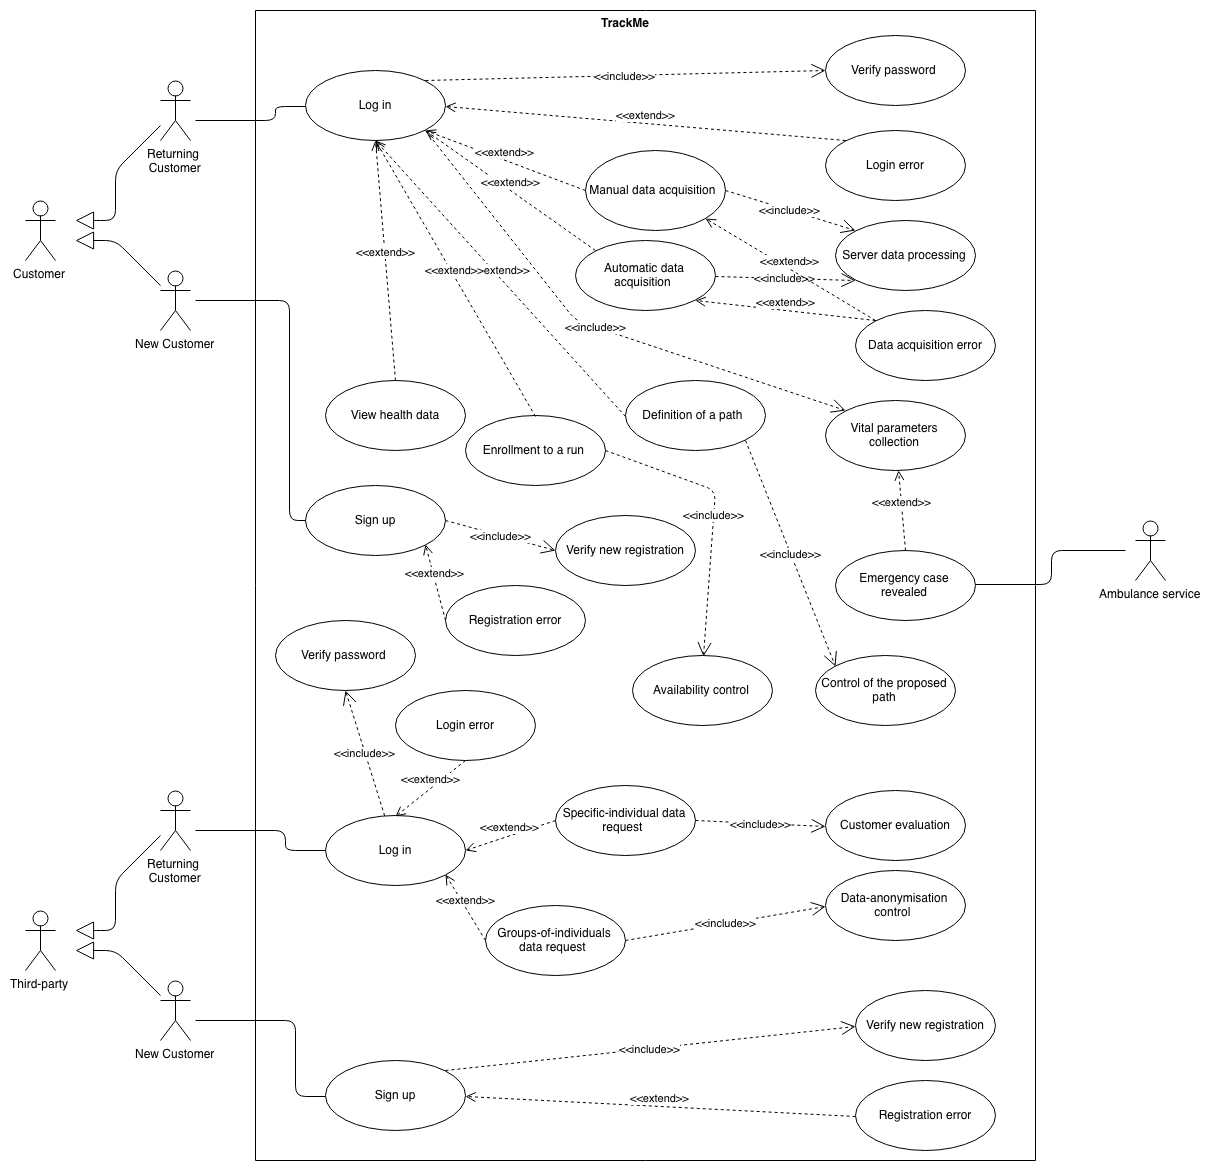
\includegraphics[width=\textwidth]{Figures/UseCaseDiagram}
  \caption{Use case diagram}
\end{figure}
\newpage

\subsection{Sequence diagrams}
\begin{figure}[h!]
  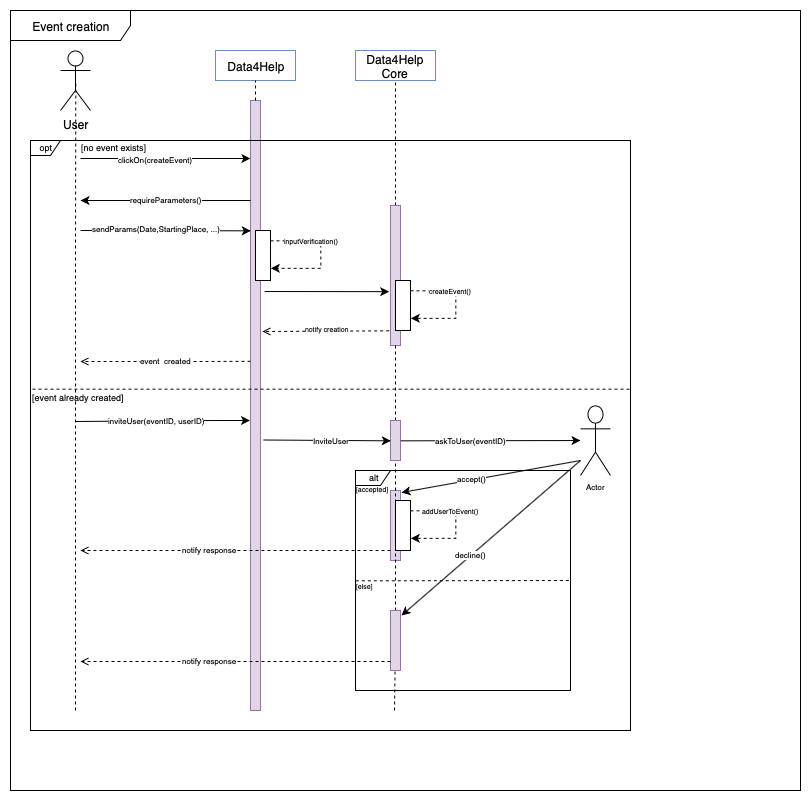
\includegraphics[width=\textwidth]{Figures/Sequence-Event}
    \caption{"Event creation and handling" sequence diagram}
\end{figure}
\newpage

\begin{figure}[h!]
  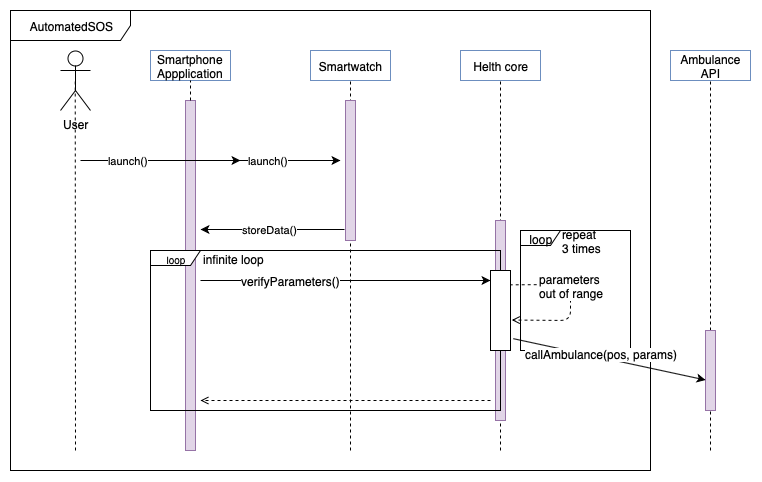
\includegraphics[width=\textwidth]{Figures/Sequence-AtomatedSOS}
  \caption{"AutomatedSOS" sequence diagram}
\end{figure}
\newpage
\begin{figure}[h!]
  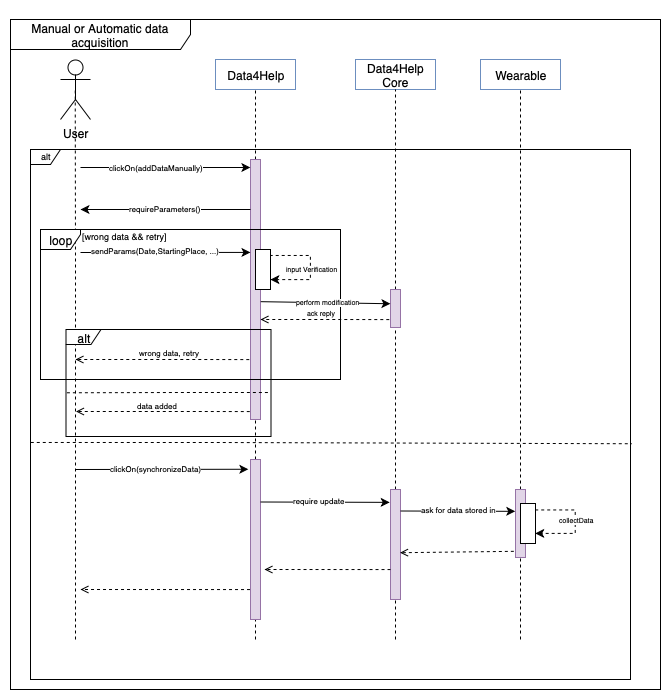
\includegraphics[width=\textwidth]{Figures/Sequence-Data}
  \caption{"Automatic/Manual data acquisition" sequence diagram}
\end{figure}
\newpage


\subsection{Performance Requirements}
	The application is designed to be consumed by Italian citizens. 
	We estimate around 30k users at app launch, with around 10\% 
	simultaneously active.
	We estimate that once the application will be brought over onto
	the Android platform, the total users count will increase by 25\%,
	topping at about 38k users.
	The application will be able to adapt to the users active 
	concurrently.

\subsection{Design Constraints}

	\subsubsection{Standards compliance}
	The software application should handle a big amount of data, 
	stored online on third-parties' servers. 
	It also should manage a great number of simultaneous requests 
	when, in example, third-parties ask to access data or during the
	period of enrolment to a run.
	
	\subsubsection{Hardware limitations}
	TrackMe is a software application available only on iOS devices. 
	It requests an internet connection (WiFi, 3G, 4G/LTE) and 
	GPS connectivity. \newline
	Some functionalities are available only for the owners of 
	wearable devices. 

	\subsubsection{Any other constraint}
	The application needs to access to the current location of the 
	user. It also may need to access individual's contact list to
	easily find possible user's friends. 
	
\newpage
\subsection{Software System Attributes}	

	\subsubsection{Reliability}
	The application and the external services offered by the
	application must be available 24/7. \newline
	Servers' maintenance, communicated to the user in advance
	and only during determined hours of the day, is the only 
	exceptions accepted. 
	
	\subsubsection{Availability}
	TrackMe services are available only in Italy for free.
	
	\subsubsection{Security}
	The security and privacy of the final user's will be guarantee by 
	TrackMe storing data and sensitive information only on encrypted 
	servers. \newline
	For online transactions, secure internet protocols are going to
	be adopted. 
	
	\subsubsection{Maintainability}
	
	
	\subsubsection{Portability}
	Portability to the Android operating system will be take into 
	consideration after a first initial phase of development dedicated
	to the iOS market. \newline
	The application will also be constantly updated to guarantee 
	compatibility to an increasing number of wearable devices. 
	
\newpage
\subsection{Scenarios}

	\subsubsection{Scenario 1}
	Tim has to sustain an important medical exam aimed to discover if 
	he suffers or not of tachycardia. He has available the latest 
	model of smartwatch that supports the EGC monitor so his doctor 
	suggests to use Data4Help to monitor for 24/48 hours his heart 
	rate. Data4Help allows Tim to just use his smartwatch, instead of 
	the classic Dynamic ECG machine, for registering his heart’s data 
	in the app so that his doctor, after committing a request to Tim 
	through his fiscal code, can examine the results after few hours 
	by the end of the test and give to Tim a response in a very short 
	time. 

	\subsubsection{Scenario 2}
	Fitness \& More is a brand new sport center situated near a very
	big residential area with many educational institutions from 
	elementary to high schools. The centre offers swimming and tennis
	lessons with expert instructors and also a well supplied gym with
	personal coaches. \newline
	Fitness \& More asks to TrackMe the access to weight and height 
	data of kids between 6 and 19 year old who live in the above 
	mentioned area to make an analysis of the presence of overweighted
	individuals and so sponsor its sport center. 

	\subsubsection{Scenario 3}
	The next PolimiRun will be held on the 11th of November in Lecco.
	Polisport, the sport organisation of the Politecnico di Milano, 
	decided to arrange a few workouts for the runners who are 
	attending the competition and so they suggest to use Track4Run to
	manage the path of the workouts around the city of Milan and also
	to let runners en-roll the training sessions. 

\newpage
\section{Formal analysis using Alloy}

In this section we give a description of the system trough and Alloy model.
The following relations are described:
\begin{itemize}
	\item Data access request system is described. Third parties can access users' data
		if a previous request has been made and approved.
	\item SOS events are raised in case of low vital parameters.
	\item Users can join to running events.
\end{itemize}
The following assumptions are taken in order to make the model cleaner:
\begin{itemize}
	\item All not necessary (to Alloy model) attributes of entities are omitted.
	\item All entities that have to be unique are identified by a single integer field: \textit{ID}.
	\item Dates are represented trough a single integer field: \textit{day}.
	\item Threshold alert value for bpm is set to 4.
\end{itemize}
\newpage
\lstinputlisting[language=alloy]{Alloy/Alloy.als}
\newpage

\begin{figure}[!h]
	\centering
	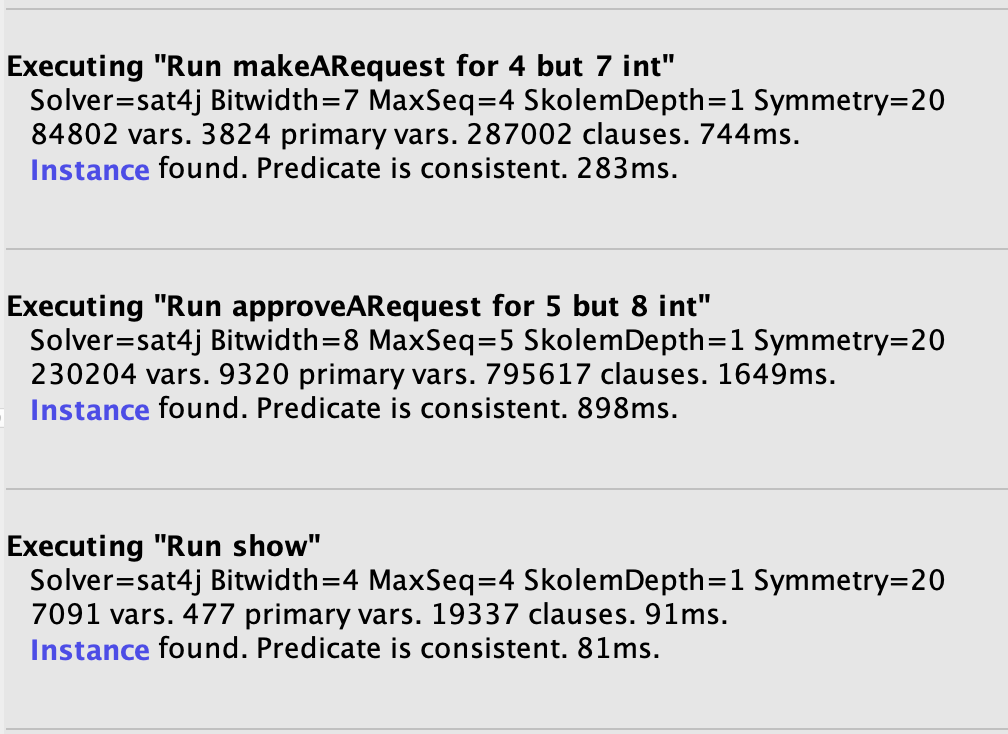
\includegraphics[height=8cm,keepaspectratio]{Figures/AlloyPredicates}
	\caption{Alloy analyser tool output.}
\end{figure}
\newpage


\subsection{World Generated}
\begin{figure}[ht]
\centering
    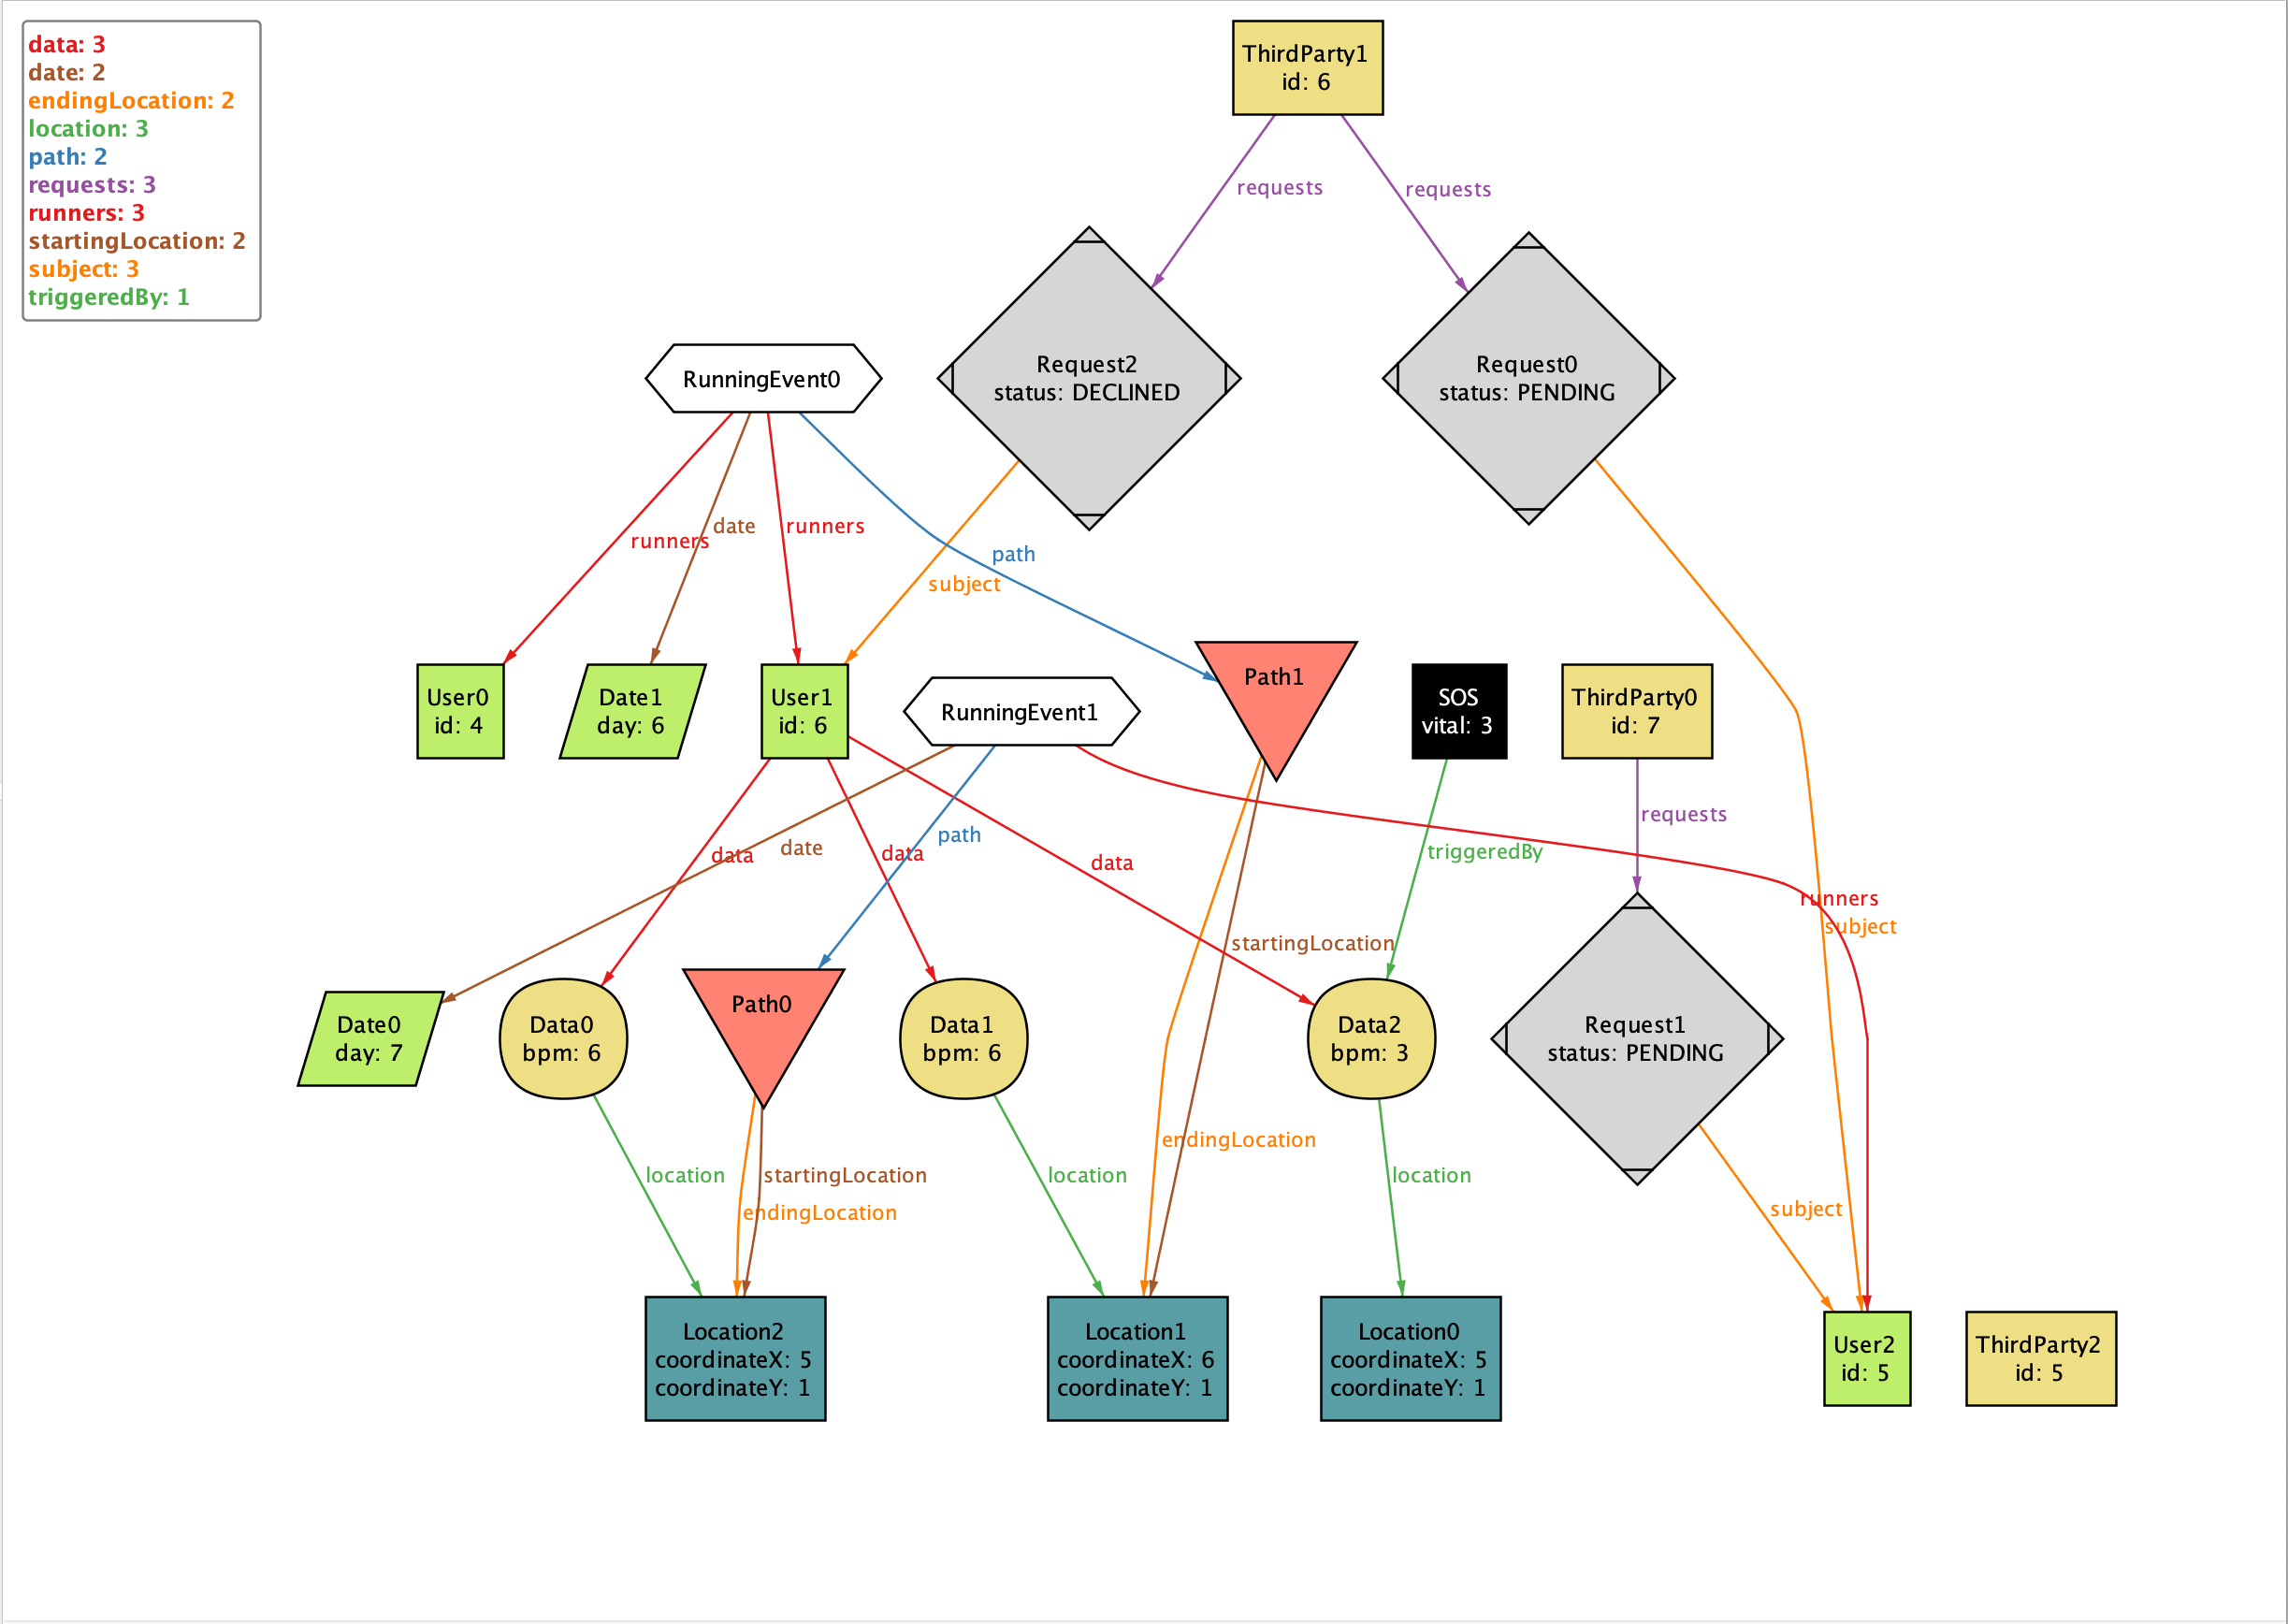
\includegraphics[height=10cm,keepaspectratio, angle=270]{Figures/AlloyWorld}
    \caption{Generated Alloy World}
\end{figure}

\newpage
\section{Effort spent}

\section{References}

\end{document}